\documentclass[12pt,handout]{beamer}
\usetheme{CambridgeUS}
\usepackage[utf8]{inputenc}
\usefonttheme{professionalfonts}
\usepackage{times}
\usepackage{tikz}
\usepackage{amsmath}
\usepackage{verbatim}
\usepackage{hyperref}
\usepackage{yfonts,color}

\usepackage{Sweavel}

\usetikzlibrary{arrows,shapes}
\defbeamertemplate{itemize item}{tikzarrow}{\tikz{\node[single
arrow,scale=0.2,inner sep=2ex,fill] at (0,0) {};}}
\author{Manuel Martin Infosol}
\title{Testing}
\subtitle{
d'après http://r-pkgs.had.co.nz/tests.html
}

\begin{document}


\begin{frame}[fragile]\titlepage
\end{frame}
%------------------------------

\begin{frame}[fragile]

Testing is a vital part of R (package) development!
\begin{center}
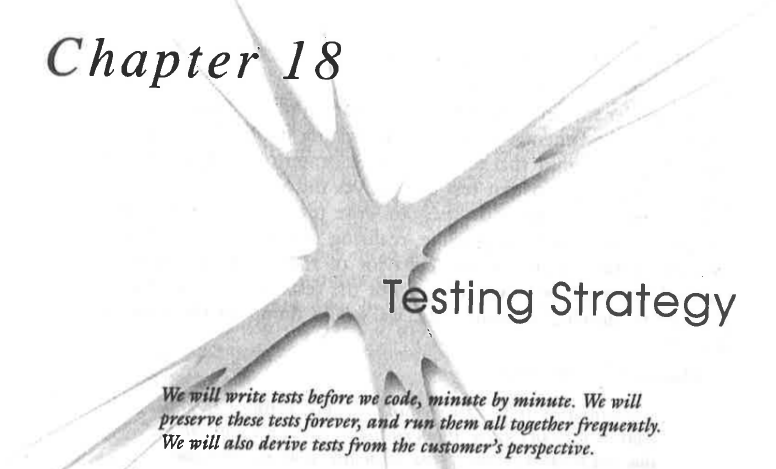
\includegraphics[width = 250pt]{../images/XPTesting.png}
\end{center}
\end{frame}
%------------------------------

\begin{frame}[fragile]
\begin{center}
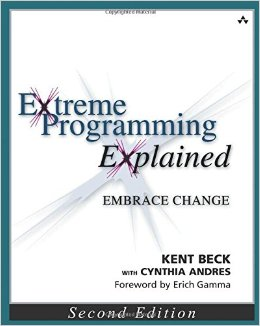
\includegraphics[width = 150pt]{../images/XP.jpg}
\end{center}

\end{frame}
%------------------------------

\begin{frame}[fragile]

Up until now, your workflow probably looks like this:

\begin{itemize}
\item Write a function.
\item Load it with Ctrl/Cmd + Shift + L or \texttt{devtools::load\_all()}.
\item Experiment with it in the console to see if it works.
\item Rinse and repeat.
\end{itemize}

%While you \_are\_ testing your code in this workflow, you're only doing it informally. The problem with this approach is that when you come back to this code in 3 months time to add a new feature, you've probably forgotten some of the informal tests you ran the first time around. This makes it very easy to break code that used to work. 

\end{frame}


%------------------------------
\begin{frame}[fragile]{Exemple : the silent bug}

\begin{Schunk}
\begin{Sinput}
> nFactorial <- function(n) {
+ 	# calculate n factorial
+ 	n_fact <- prod(1:n)
+ 
+ 	return(n_fact)
+ }
> nFactorial(12)
\end{Sinput}
\begin{Soutput}
[1] 4.79e+08
\end{Soutput}
\end{Schunk}
\end{frame}
%------------------------------

\begin{frame}[fragile]
\begin{Schunk}
\begin{Sinput}
> prod <- function(v){
+ 	res <- 1
+ 	for (el in v) res <- res * el * 2
+ 	return(res)
+ }
\end{Sinput}
\end{Schunk}

\begin{Schunk}
\begin{Sinput}
> nFactorial(12)
\end{Sinput}
\begin{Soutput}
[1] 1.962e+12
\end{Soutput}
\end{Schunk}
\end{frame}
%------------------------------


\begin{frame}[fragile]{Why testing pays off}
\begin{itemize}

\item Fewer bugs. Because you're explicit about how your code should behave
  you will have fewer bugs.

\item  By following this approach to testing, you can be sure that bugs 
  that you've fixed in the past will never come back to haunt you.

\item Better code structure (modular). Code that's easy to test is usually better designed.

\item Easier restarts.

\item Robust code. If you know that all the major functionality of your package has 
  an associated test, you can confidently make big changes without worrying 
  about accidentally breaking something.

\end{itemize}


\end{frame}
%------------------------------



\begin{frame}[fragile]
Tests are organised hierarchically: \textit{expectations} are grouped into \textit{tests} which are organised in \textit{files}:

\begin{itemize}
\item An \textit{expectation} is the atom of testing. It describes the expected result 
  of a computation: Does it have the right value and right class? Does it 
  produce error messages when it should? Expectations are functions that start 
  with \texttt{expect\_}.

\item A \textit{test} groups together multiple expectations to test the output
  from a simple function. This is why they are sometimes called \textit{unit}
  as they test one unit of functionality. A test is created with \texttt{test\_that()} .

\item A \textit{file} groups together multiple related tests. Files are given a human 
  readable name with `context()`.

\end{itemize}


\end{frame}
%------------------------------

\section{Expectations}

\begin{frame}[fragile]{expect\_}

An expectation is the finest level of testing and all expectations have a similar structure:

\begin{itemize}
\item They start with \texttt{expect\_}.

\item They have two arguments: the first is the actual result, the second is what 
  you expect.
  
\item If the actual and expected results don't agree, testthat throws an error.

\end{itemize}
There are almost \textbf{20} expectations in the testthat package.

\end{frame}
%------------------------------


\begin{frame}[fragile]{expect\_equal and expect\_identical}

\texttt{expect\_equal()} is the most commonly used: it 
    uses `all.equal()` to check for equality within a numerical tolerance:

\begin{Schunk}
\begin{Sinput}
>     expect_equal(10, 10)
>     expect_equal(10, 10 + 1e-7)
>     expect_equal(10, 11)
\end{Sinput}
\end{Schunk}
  
For exact equivalence, or need to compare a more exotic object like an environment, 
use \texttt{expect\_identical()}.

\begin{Schunk}
\begin{Sinput}
>     expect_equal(10, 10 + 1e-7)
>     expect_identical(10, 10 + 1e-7)
\end{Sinput}
\end{Schunk}

\end{frame}
%------------------------------


\begin{frame}[fragile]{expect\_match}
\texttt{expect\_match()} matches a character vector against a regular expression. 
    The optional `all` argument controls whether all elements or just one 
    element needs to match.

\begin{Schunk}
\begin{Sinput}
>     string <- "Testing is fun!"
>     expect_match(string, "Testing") 
>     # Fails, match is case-sensitive
>     expect_match(string, "testing")
>     # Additional arguments are passed to grepl:
>     expect_match(string,"testing",ignore.case = TRUE)
\end{Sinput}
\end{Schunk}

\end{frame}
%------------------------------


\begin{frame}[fragile]{variations of expect\_match}
Four variations of \texttt{expect\_match()} let you check for other types of 
    result: \texttt{expect\_output()}, inspects printed output;     
\begin{Schunk}
\begin{Sinput}
>     a <- list(1:10, letters)
>     expect_output(str(a), "List of 2")
>     expect_output(str(a), "int [1:10]", fixed = TRUE)
\end{Sinput}
\end{Schunk}
\end{frame}
%------------------------------


\begin{frame}[fragile]{Other variations, testing warnings and failures}
\begin{Schunk}
\begin{Sinput}
>     expect_message(message("salut"))
\end{Sinput}
\end{Schunk}
    
%    With \texttt{expect\_message()}, \texttt{expect\_warning()}, \texttt{expect\_error()} you can
%    leave the second argument blank if you just want to see if a message,
%    warning or error is created. However, it's normally better to be explicit, 
%    and provide some text from the message.
%


\begin{Schunk}
\begin{Sinput}
>     expect_message(message("Hi!"), "bonjour.")    
>     expect_warning(log(-1))
>     # But always better to be explicit
>     expect_warning(log(-1), "NaNs produced")
>     # Failure to produce a warning or error when an error is expected
>     expect_warning(log(0))
>     expect_error(1 / 'a') 
\end{Sinput}
\end{Schunk}
\end{frame}
%------------------------------


\begin{frame}[fragile]
\texttt{expect\_is()} checks that an object `inherit()`s from a specified class.

\begin{Schunk}
\begin{Sinput}
>     model <- lm(mpg ~ wt, data = mtcars)
>     expect_is(model, "lm")
>     expect_is(model, "glm")
\end{Sinput}
\end{Schunk}

\end{frame}
%------------------------------


\begin{frame}[fragile]{Cache it!}
Sometimes you don't know exactly what the result should be, or it's too 
    complicated to easily recreate in code. In that case the best you can do is 
    check that the result is the same as last time. \texttt{expect\_equal\_to\_reference()} 
    caches the result the first time its run, and then compares it to subsequent 
    runs. If for some reason the result does change, just delete the cache (*)
    file and re-test.

\end{frame}
%------------------------------


\begin{frame}[fragile]{}

\section{Writing tests}

Each test should have an informative name and cover a single unit of functionality. 

$\rightarrow$ You create a new test using \texttt{test\_that()}, with test name and code block as arguments.

$\rightarrow$ The message associated with the test should be informative so that you can quickly narrow down the source of the problem.

\end{frame}
%------------------------------


\begin{frame}[fragile]{cleaning Up}

Each test is run in its own environment and is self-contained. However, testthat doesn't know how to cleanup after actions affect the R landscape: 

\begin{itemize}
\item The filesystem: creating and deleting files, changing the working directory,
  etc.

\item The search path: `library()`, `attach()`.

\item Global options, like `options()` and `par()`.

\end{itemize}



\subsection{What to test}
\end{frame}
%------------------------------


\begin{frame}[fragile]{What to test}

\textit{Whenever you are tempted to type something into a print statement or a 
debugger expression, write it as a test instead.}--- Martin Fowler

\end{frame}
%------------------------------


\begin{frame}[fragile]{What to test}
There is a fine balance to writing tests. 

\begin{itemize}
\item Focus on testing the external interface to your functions.

\item Strive to test each behaviour in one and only one test.

\item Avoid testing simple code that you're confident will work.

\item Always write a test when you discover a bug.

\end{itemize}

\end{frame}
%----------------

\section{Test workflow for package creation}
\begin{frame}[fragile]
To set up your package to use testthat, run, from the package's directory:

\begin{Schunk}
\begin{Sinput}
> devtools::use_testthat()
\end{Sinput}
\end{Schunk}

% use the forest package?

This will:
\begin{itemize}

\item  Create a \texttt{tests/testthat} directory.

\item  Adds \texttt{testthat} to the \texttt{Suggests} field in the \texttt{DESCRIPTION}.

\item  Creates a file \texttt{tests/testthat.R} that runs all your tests when
    \texttt{R CMD check} runs. (You'll learn more about that in \textit{automated checking}
\end{itemize}

\end{frame}
%------------------------------



\begin{frame}[fragile]
Once you're set up the workflow is simple:

\begin{itemize}
\item  Modify your code or tests.

\item  Test your package with Ctrl/Cmd + Shift + T (RStudio) or \texttt{devtools::test()}.

\item  Repeat until all tests pass.

\end{itemize}


\end{frame}
%------------------------------



\begin{frame}[fragile]
The testing output looks like this:

    Expectation : ........... \\
    rv : ... \\
    Variance : ....123.45. \\

Each line represents a test file. Each `.` represents a passed test. Each number represents a failed test. 

\end{frame}
%------------------------------



\begin{frame}[fragile]
The numbers index into a list of failures that provides more details:
\begin{itemize}

    \item \texttt{Failure(@test-variance.R): Variance correct for discrete uniform rvs -----
    VAR(dunif(0, 10)) not equal to var\_dunif(0, 10)
    Mean relative difference: 3}
    
    \item \texttt{Failure(@test-variance.R): Variance correct for discrete uniform rvs -----
    VAR(dunif(0, 100)) not equal to {var\_dunif(0, 100)}
    Mean relative difference: 3.882353}

\end{itemize}

Each failure gives a description of the test (e.g., "Variance correct for discrete uniform rvs"),
 its location (e.g., "\@test-variance.R"), and the reason for the failure (e.g., "VAR(dunif(0, 10))
 not equal to var\_dunif(0, 10)"). The goal is to pass all the tests.
\end{frame}
%------------------------------



\begin{frame}[fragile]{\texttt{test-} files}
A test file lives in `tests/testthat/`. Its name must start with `test`. 


\begin{itemize}
\item The highest-level structure of tests is the file. 
\item Each file should contain a single `context()` call that provides a brief description of its contents. 
\end{itemize}
\end{frame}

%------------------------------


\end{document}
